\documentclass[hidelinks,12pt]{article}
\linespread{1.3}
\usepackage{hyperref}
\usepackage{enumerate,changepage,lipsum,titlesec}
\usepackage{cite}
\usepackage{comment, xcolor}
\usepackage[pdftex]{graphicx}
  \graphicspath{{images/}, {images/stat/}}
  \DeclareGraphicsExtensions{.pdf,.jpeg,.png, .jpg}
\usepackage[cmex10]{amsmath}
\usepackage{array} 
\usepackage{subfigure} 
\newcommand{\grey}[1]{\textcolor{black!30}{#1}}
\newcommand{\red}[1]{\textcolor{red!50}{#1}}
\newcommand{\fref}[1]{Figure \ref{#1}}
\newcommand{\tref}[1]{Table \ref{#1}}

\oddsidemargin0cm
\topmargin-2cm %I recommend adding these three lines to increase the
\textwidth16.5cm %amount of usable space on the page (and save trees)
\textheight23.5cm

\makeatletter
\renewcommand\paragraph{\@startsection{paragraph}{4}{\z@}%
            {-2.5ex\@plus -1ex \@minus -.25ex}%
            {1.25ex \@plus .25ex}%
            {\normalfont\normalsize\bfseries}}
\makeatother
\setcounter{secnumdepth}{4} % how many sectioning levels to assign numbers to
\setcounter{tocdepth}{4}    % how many sectioning levels to show in ToC


\begin{document}
\title{Dynamic Energy Mapping Project Outline}
\maketitle
\tableofcontents
\newpage
\section{General Introduction}
\subsection{Project Overview}
Buildings alone account for 40\% of the total energy usage in the
United States. However if the indirect energy impact of the built
environment as a whole was considered, the community design induced
energy and environmental impact could exceed this already high ratio:
60\% - 75\% of the energy consumption is connected to the spatial
layout of built environment~\cite{Owens199281}. In a broader sense,
the energy resources distribution influences the layout of human
activities~\cite{Owens199281}. More specifically, built environment
influence the energy throughput in the form of land use design and
infrastructure layout~\cite{Jaccard19971065}. 

Community Energy Management (CEM) is a combination of community level
design strategies and energy management strategies aiming at providing
quality of life in an urban environment with minimized energy
consumption and environmental impact~\cite{Jaccard19971065}. It
contains ``land use planning'', ``transportation management'', ``site
planning'' and ``local energy supply and delivery planning''~\cite{Jaccard19971065}.

Energy Mapping makes the community energy planning alternatives
visible to planners and policy makers~\cite{baird2014}. Energy Map, or
energy master plan~\cite{londonHeatMap} contains the information of
energy demand and supply in the form of energy
intensity~\cite{baird2014}, renewable energy, residual
energy~\cite{Dobbelsteen2013} and decentralized energy
network~\cite{decentralHeatMap2011}. It facilitates the matching of
energy demand and supply in the aspect of spatial, temporal and
quality ~\cite{Dobbelsteen2013}. 

The current challenge of the Energy Mapping approach is its lack of
temporal information of energy supply and demand, creating barriers
for the matching of demand and supply in the a time-of-use
fashion~\cite{baird2014}.

A Dynamic Energy Map aggregates the time-of-use energy information to
the traditional Energy Mapping practices. It acts as a geo-database
that holds 1) hourly energy profile data for each building and the
aggregated energy profile data for the whole community; 2) hourly
energy supply data of community decentralized energy
sources~\cite{baird2014}. With the Dynamic Energy Map, the temporal
behavior of the demand and supply of heating, cooling and electricity
are revealed and are available to be compared, analyzed and
updated. Dynamic Energy Map is also connected to simulation software,
and can act as a key component of Geo-design that encompasses
``geo-spatial modeling, impact simulations, and real-time feedback to
facilitate holistic designs and smart
decisions''~\cite{esriGeodesign2012}. The development of data-driven
approaches and machine learning methods could also be coupled and can
perform more complicated analysis of spatial-temporal behavior of
energy data and provide more informative design or management support.

\subsection{Objective and Problem Definition}
The objective of the project is to 1) implement a Dynamic Energy
Demand Map with hourly thermal energy consumption data for each
building and the whole community 2) use it to optimize the arrangement
of land use pattern to improve the energy performance in terms of
aggregated thermal energy demand variation and 3) support sizing of a
district thermal energy supply system.

The community model is created in City Engine~\cite{cityEngine2015}
based on the land use pattern of a mixed-use redevelopment project at
Lower Hill District, Pittsburgh, PA~\cite{Ramesh2013}. The model
contains 68 buildings, comparable to a typical service area of a
district thermal energy system (combined heating and cooling), about
50 to 150 buildings~\cite{IDEA2005}.

The hourly heating (gas) and cooling energy (electricity) consumption
profile is retrieved from DOE Commercial Benchmark Building
simulation~\cite{DOE2015}. An interface was designed to combine the
8760 heating-cooling energy choropleth map images from City Engine and
the 8760 hourly heating-cooling energy data from EnergyPlus to form a
Dynamic Energy Map. The interface provides users with the functions of
1) navigating through the dynamic map images, 2) dynamic data
plots of single buildings, building sectors and aggregated community
thermal energy demand.

\subsection{Related Concepts}\label{concept}
Some related key concepts will be discussed in this section include
district energy system, Energy Map and Dynamic Energy Map.

\subsubsection{District Thermal Energy System}
A Decentralized Energy System is a ``local or sub-regional supply of
energy from a local source.''~\cite{lhmreport2012}. It brings the
energy generation near to the energy end users and reduces the energy
transmission and distribution loss~\cite{decentralHeatMap2011}. A
district energy system is one form of decentralized energy
generation. It can produce thermal energy in a central plant and
deliver the thermal energy to local buildings through a closed-loop
pipeline network. Thermal energy are delivered in the form of steam,
hot water or chilled water~\cite{baird2014}. The central power plant
can take on one of the following forms: 1) thermal power plant that
only generates thermal energy, which can be either heating or cooling
energy 2) co-generation system, or combined heat and power (CHP)
system, that generates electricity and reuses the reject heat from
electricity generation to serve space heating and service hot water to
local buildings~\cite{IDEA2005} 3) tri-generation system, where the
central plant uses the heat generated by CHP plant to produce chilled
water and supply both heating and cooling energy
~\cite{cchp2015}. Corresponding to the different types of power plant,
the network delivering thermal energy can be classified as 1) district
heating network that only delivers steam or hot water 2) district
thermal network that delivers both heating energy in the form of
steam or hot water and cooling energy as chilled water.

There are several advantages of adopting a district thermal energy
system: the central power plant can use a broader range of fuel
choices including natural gas, oil, coal, waste, and renewable energy
sources in the generation of thermal energy. This makes the district
thermal energy system more flexible and more competitive in the market
and increases the energy system resilience~\cite{IDEA2005}. It reduces
the transmission loss of thermal or power (if the central plant is a
CHP plant or CCHP plant) by bringing energy production closer to
energy end use~\cite{decentralHeatMap2011}. It has high energy
generation efficiency as a result 1) it can utilize high efficiency
large-scale energy generation equipment and 2) it provides better
``load matching''~\cite{IDEA2005}. It also reduces the space and cost
dedicated to installation and maintenance of HVAC systems in single
buildings and reduces harmful gas emission~\cite{IDEA2005}.

\subsubsection{Heat Map}
Heat map is defined as ``a spatial plan of existing and planned
building heat demand, and decentralised energy networks and generation
equipment''~\cite{decentralHeatMap2011}. It is also a GIS ``live
database'' that allows new development information to be
incorporated. It is a key component to the DE energy master
plan~\cite{decentralHeatMap2011}.

\subsubsection{Energy Map}
Energy Map is a generalization of a heat map that includes energy
supply, demand and infrastructure information of various energy forms
and technologies. It is also a combination of building energy
database, a subset of the BIM (Building Information Model), and a
Geo-database or Geographical Information System (GIS). 

Energy Map can help to envision the community or city level energy
demand reduction with high performance building
design~\cite{aacip2009}. It can be used in supporting district heating
system design~\cite{decentralHeatMap2011, Finney2012165} by
visualizing the heat sources and sinks.

\subsubsection{Dynamic Energy Map}
Dynamic Energy is a Energy Map equipped with temporal information of
energy supply and demand. It enables spatial-temporal comparison,
aggregation and query of energy demand and supply. When coupled with
Energy simulation tools, design alternatives would be evaluated and
compared at each given time spot or time period. By performing
advanced data analysis method, the dynamic map makes patterns that are
omitted in static maps visible and analyzable. Both aspects enable
more detailed energy analysis and design support.

\subsection{Why ``time'' dimension is important for an Energy Map}
\subsubsection{Strong Temporal Variation of Energy Demand}
Different building types often indicates different energy demand
profile. For example, the residential building heat demand profile has
two major peaks, morning and evening, and is relatively low for the
rest of the day. For office buildings, there is a peak heat demand in
the morning and a relatively high heat demand through the day time but
drops in the evening. Hospitals usually have a more flattened demand
throughout the day. Within a mixed-used urban environment, the arrival
of peak demand for different buildings are usually not
simultaneous~\cite{decentralHeatMap2011}.

In the design of a district energy system, mixing building types with
different time-of-use energy profile can be helpful in creating a less
variate aggregated energy demand. This allows the central power plant
in a district thermal energy system to a have higher utilization rate
and reduces the need for backup plant that accounts for high peak
demand~\cite{decentralHeatMap2011}.

\begin{figure}[h!]
  \centering
  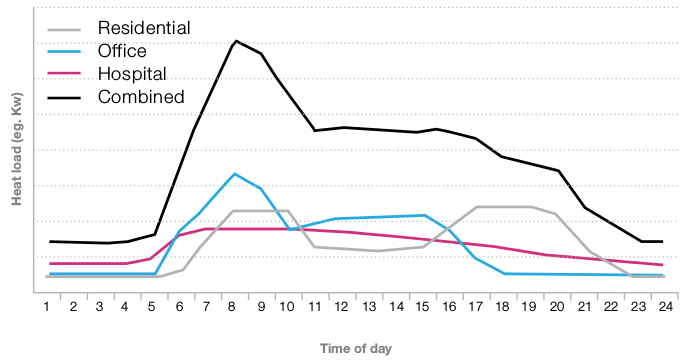
\includegraphics[width=0.7\linewidth]{mixLoad.png}
  \caption{Mixing Load of Different Building
    Type~\cite{decentralHeatMap2011}}
  \label{fig:mixLoad}
\end{figure}

\subsubsection{Aggregation of Peak Value Becomes Tricky for Data with Time Variation}
One common mistake for sizing a district thermal energy system is to
add up the peak demand of each terminal users. Since the peak demand
of individual buildings do not occur at the same time, the end result
of summing up the peak demand at each end point exceeds the actual
total demand peak of the community, hence with this approach, the
whole district system becomes excessively over-sized, which reduces
the whole system efficiency. Dynamic Energy Map can reveal the problem
of such approaches by directly providing the aggregated thermal energy
demand for the community and for single buildings or building
sectors. It allows a side by side comparison of single building demand
and aggregated demand and eliminates the misunderstanding of the
demand aggregation. With the direct information of aggregated thermal
energy demand, it also assists actually sizing a district thermal
energy system.

\newpage
\section{Related Works}
Section \ref{staticEnergyMap} and section \ref{dynamicMap} provide an
overview of the existing instances of static energy maps and dynamic
energy maps. Section \ref{mapDesign} and \ref{stDataAnalysis} provides
some supporting evidences for certain design choices. Section
\ref{4dMap} provides some information on potential technologies for
further development. \grey{(?? are not written)}

\subsection{Static Energy Map}\label{staticEnergyMap}
\subsubsection{Calgary Energy Map}
One of the early instances of Static Energy Mapping practices is the
Energy Mapping Study of City of Calgary in 2008, carried out by
Canadian Urban Institute. It aims at providing insights to achieve
the goal of reducing 50\% of Green House Gas (GHG) emissions by
2050~\cite{aacip2009}. It depicts 1) how building design strategies
and land use planning can influence the city level energy use
intensity 2) the availability of alternative energy sources and the
opportunities to combine building level sustainable design technology
with the community level energy system design. 

Calgary energy map first compares energy use intensity (the annual
total demand for thermal energy of space heating cooling, hot water
and electricity per unit area~\cite{aacip2009}) in GJ/ha between two
development cases: ``business as usual'' case and ``ultra-high
efficiency'' case (\fref{fig:calgaryCmp}). The comparison demonstrated
a 34\% reduction in energy use intensity from the former to the
latter~\cite{aacip2009}.

\begin{figure}[h!]
  \centering
  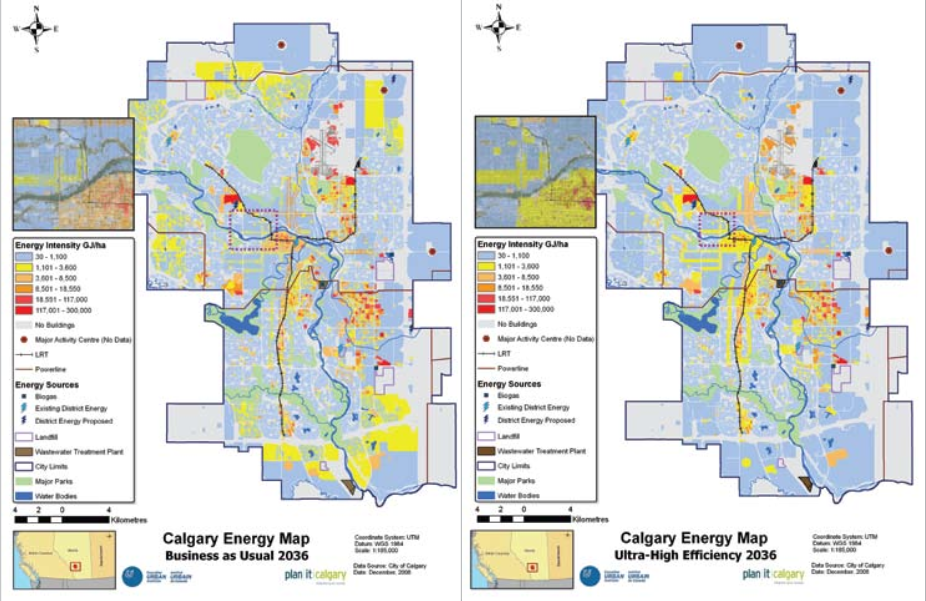
\includegraphics[width=0.6\linewidth]{calgaryCmp.png}
  \caption{Calgary Energy Map (Business as Usual, Ultra-High
    Efficiency)~\cite{aacip2009}}
  \label{fig:calgaryCmp}
\end{figure}

It also shows alternative energy sources of district energy, solar hot
water, solar air, energy sharing and PV installation on the map
(\fref{fig:calgaryAlter}). By overlaying the alternative technology
map and the ``ultra-high efficiency'' map, it highlights the
opportunities of using alternative renewable energy sources and
district energy system to further improve the energy performance of
high energy demand areas after high performance building design was
applied~\cite{aacip2009}.

\begin{figure}[h!]
  \centering
  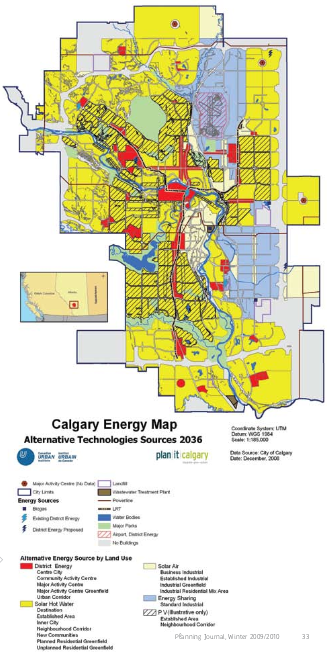
\includegraphics[width=0.3\linewidth]{calgaryAlter.png}
  \caption{Calgary Energy Map Alternative Energy Source~\cite{aacip2009}}
  \label{fig:calgaryAlter}
\end{figure}

\subsubsection{UK Heat Map}
Under the goal of supplying 25\% of the total energy with
decentralized energy (DE) by the year 2025, the Decentralised Energy
Master Planning Program (DEMaP) was conducted between 2008 to 2010 to
``identify opportunities for district heating networks through heat
mapping and energy masterplanning''~\cite{londonHeatMap}. In this
study, the term DE only refers to ``combined heat and power systems
connected to district heating
networks''~\cite{decentralHeatMap2011}. 

London Heat Map is a publicly accessible interactive map developed as
part of the DEMaP project. It is completed for the London Boroughs in
2012. It can act as a starting point of Energy Master Plan for local
authorities, and can assist developers to make connections to existing
DE networks to meet policy requirements (London Plan DE
policy)~\cite{decentralHeatMap2011, londonHeatMap}. Point features of
high heating energy consumers and suppliers, existing and emerging
energy networks are depicted on the interactive map. High DE potential
regions (``focus area''~\cite{decentralHeatMap2011}) are identified
and depicted on the map to highlight the opportunities of utilizing
the heat supply in the community planning and development
(\fref{fig:londonHeat}). The ``live-database'' property of London Heat
Map allows new data of energy consumption be uploaded by users.

The criteria applied for identifying focus area include: 1) near to
existing or emerging DE network, 2) high heat demand density 3) anchor
load building, 4) diverse heating demand profile 5) has public
ownership with policy concerns to make connections to the DE
network~\cite{decentralHeatMap2011}. The physical constraint are also
considered in finalizing the high DE potential regions.
\begin{figure}[h!]
  \centering
  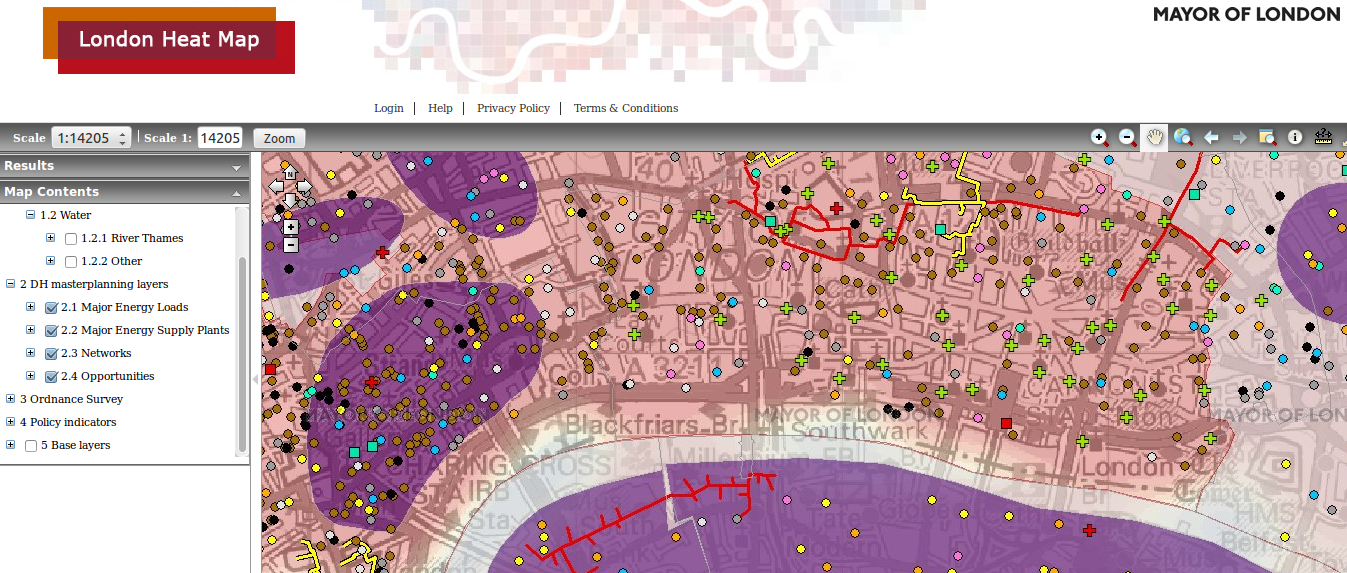
\includegraphics[width=0.7\linewidth]{londonHeat.png}
  \caption{London Heat Map~\cite{londonHeatMapMap}}
  \label{fig:londonHeat}
\end{figure}

National Heat Map (\fref{fig:nhm}) is another UK energy mapping
project that focuses more on the industry
side~\cite{decentralHeatMap2011}. It is a ``high resolution
web-based'' heating energy interactive map, developed by the
Department of Energy and Climate Change (DECC). It aims at ``support
planning and deployment of local low-carbon energy projects in
England''~\cite{heatMap2015}. Power plant developers can use this map
to consider the feasibility for a CHP plant under policy
requirements~\cite{decentralHeatMap2011}. Heating demand density
($kWh/m^2$) of four major building sectors: public buildings,
commercial buildings, industry buildings and residential buildings,
together with the total demand is plotted on the map as a 2D raster
image with a discrete color scheme from blue to red representing low
to high heating demand. Heat source of CHP stations and thermal power
stations are plotted as point features in the map. Address level heat
demand data in csv format is also available for local authorities upon
request~\cite{heatMapLocal2012}.

\begin{figure}[h!]
  \centering
  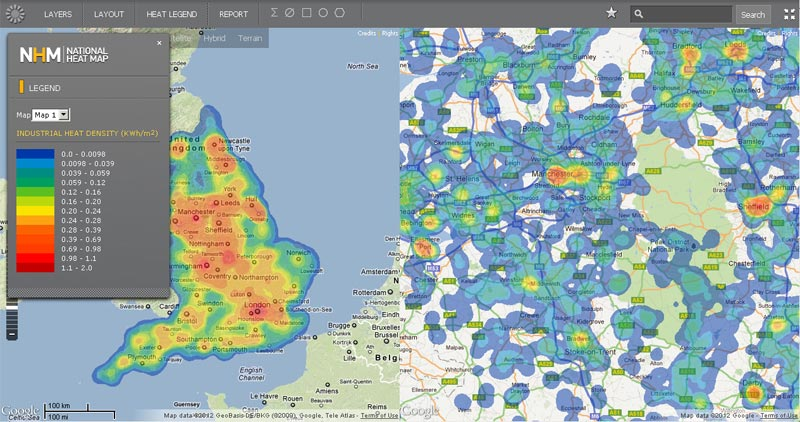
\includegraphics[width=0.5\linewidth]{nhm.jpeg}
  \caption{National Heat Map~\cite{heatMap2012}}
  \label{fig:nhm}
\end{figure}

The ``Water Source Heat Map'' (\fref{fig:waterMap}) is an added layer
group to the existing National Heat Map with information about the the
heat potential of the 4041 waterways in England. Heat potential of
waterways are represented in temperature, surface area, flow rate and
heat capacity ($kJ/m^3$ for coastal and estuary, $kW$ for canal, river
and settlement). It aims at supporting the plan of water-based thermal
system as water-based heat pump~\cite{waterHeatMap}. The map revealed
the large thermal capacity of water bodies that could serve over one
million buildings in the UK~\cite{waterHeatMap}.

\begin{figure}[h!]
  \centering
  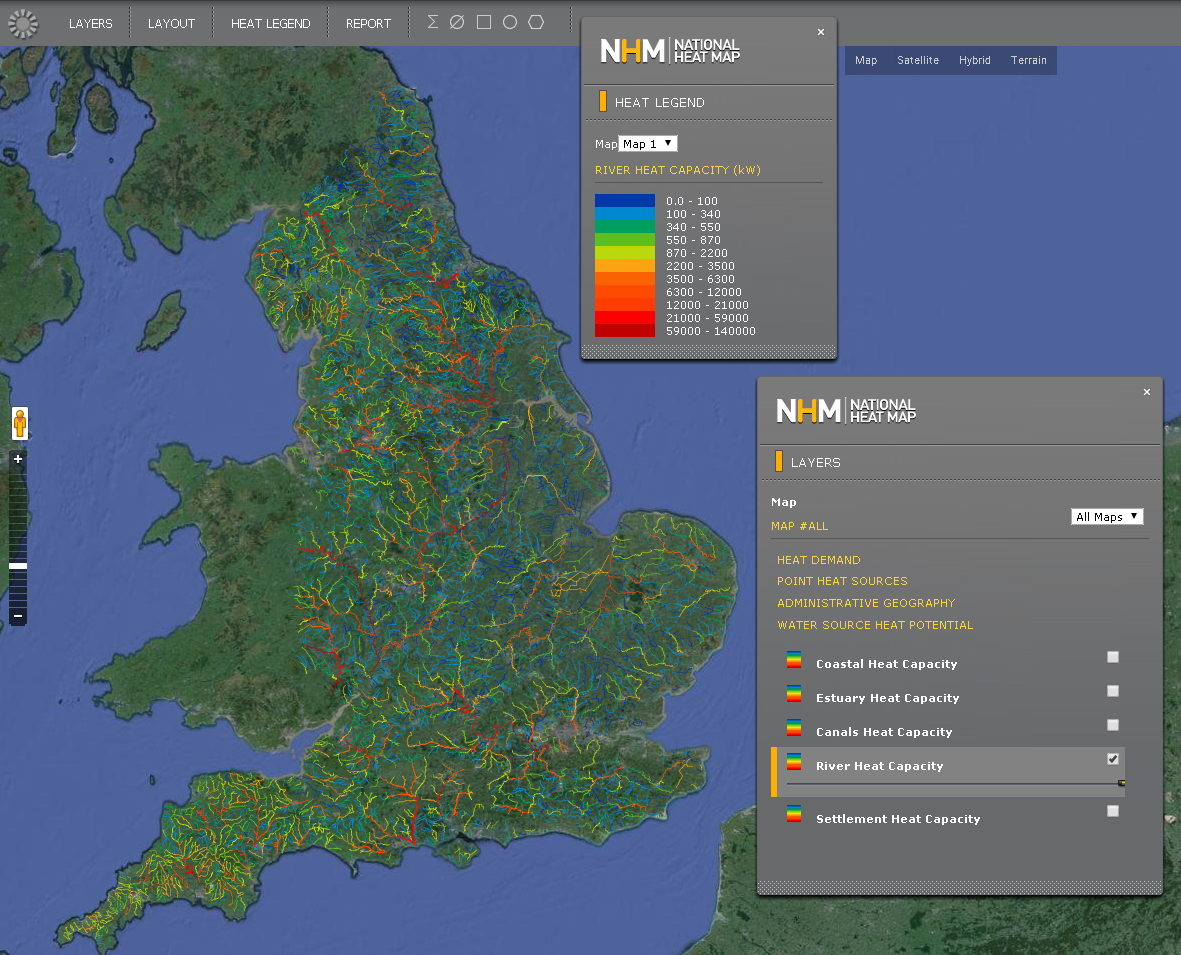
\includegraphics[width=0.5\linewidth]{waterMap.png}
  \caption{Water Heat Map~\cite{waterHeatMap}}
  \label{fig:waterMap}
\end{figure}

\subsubsection{Energy Potential Mapping}
Dobbelsteen et al. described a framework of Energy Potential Mapping
(EPM) that aggregates information of energy supply, demand and
infrastructure on the same map with demand and supply represented in
the same unit of GJ or GJ/ha~\cite{Dobbelsteen2013}.

In 2010, a ``Heat Mapping'' study under the framework of EPM was
launched by TU Delft aiming at visualizing heat demand and supply and
infrastructure with the same unit that facilitates easy comparison and
facilitates the matching of supply and
demand~\cite{Dobbelsteen2013}. The map is presented with aggregated
supply and demand in a 3D Heat Map. The absolute quantity of each type
of demand and supply is represented with extruded height in the 3D
map. Demand is represented with a transparent 3D feature, and each
supply source is represented with solid 3D feature in a different
color~\cite{Dobbelsteen2013}.

\begin{figure}[htbp]
  \centering
  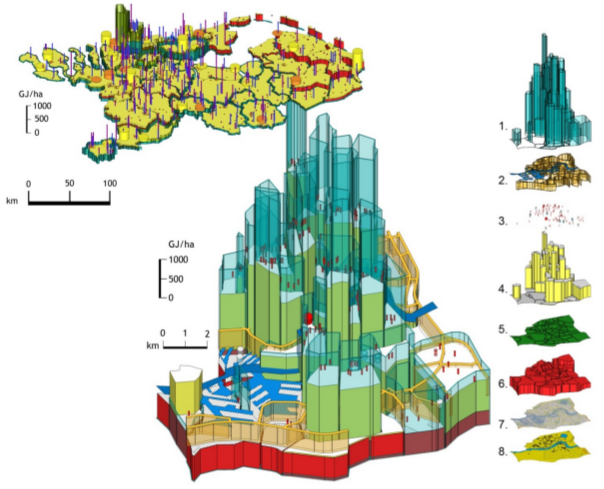
\includegraphics[width=0.7\linewidth]{heatmapNL.png}
  \caption{Heat Mapping of Netherlands and
    Rotterdam~\cite{Dobbelsteen2013}}
  \label{fig:heatmapNL}
\end{figure}

\begin{comment}
\subsubsection{Supply}
\paragraph{Assessing Renewable Energy Potential}
Voivontas et al. developed a decision support tool using GIS for
accessing the wind energy potential in four aspects: the theoretical
potential in terms of wind speed, availability potential in terms of
land use regulations, technological potential in terms of energy
production features of wind turbine and economical potential in terms
of IRR. 

``NYC City Solar Map'' presents solar energy potential for
buildings across the New York city. The map presents solar energy
generation curve, estimated solar system installation area, financial
incentive and payback~\cite{NYCSolarMap}

Other efforts tackles multiple renewable energy sources:

Ramachandra and Shruthi produced a series of district level renewable
energy theoretical potential maps of solar, wind, hydroenergy and
biomass in Karnataka State, India. The potential is estimated based on
data of global solar radiation, wind speed, hydropower plant capacity,
and plantation and livestock information. GIS is used in aggregating
energy potential data to each district. Each type of renewable energy
source is presented as a univariate thematic energy map.

\subsubsection{Demand and Infrastructure}
\paragraph{Analysis or design support of existing energy
  infrastructures}\label{infra}

\paragraph{Energy consumption prediction model}
Kolter and Ferreira presented a modeling method to predict building
energy end use in Cambridge, MA. They also developed a user
application, ``Energy View'' with two target user groups: general
public and local authorities. The model can be used by local
authorities to identify energy usage outliers and by general public to
compare their monthly energy consumption with predicted baseline
consumption. 

This case suggested how Dynamic Energy Map as a database can be
combined with more complicated data analysis method that reveals more
detailed spatial-temporal pattern. Their current time resolution of
the energy consumption data prediction is on month. If the resolution
increases to hour, the model could then be used to 1) assist better
supply side control of energy generation 2) help individual users to
better understand their energy usage behavior and provide more specific
suggestions about energy saving behavior.

\paragraph{Smart Management of Urban Energy System}
Energy Map also helps smart management of energy system in a large
urban scale. ``Smart Urban Services for Higher Energy Efficiency''
(SUNSHINE) project is a European Co-Founded energy mapping project
launched in 2013. The application is accessible through web page and
smart phone or tablet application. It aims at developing a platform
capable of 1) assessing building energy consumption behavior and
create a 2D and 3D energy map, ``ecomap'' accordingly 2) providing
automatic alerts regarding optimized usage of heating/cooling system
3) remote control of public building lighting
systems~\cite{SUNSHINE2015}. The target users of the application
include facility managers, policy makers, citizens and energy service
companies. Function 1) is anticipated to help energy company and
facility managers to identify energy consuming outliers, provide
information for building pre-certification. Function 2) aims at
providing more accurate baseline consumption data using weather and
meter data. Function 3) allows better management of public lighting
system based on illuminance requirements and weather conditions.

\subsubsection{Combined Supply, Demand and Infrastructure}
\subsubsection{Reflections}\label{Reflection}
The existing mapping approaches had their main effort in the data
calculation and aggregation, however the resulted visual
representation is questionable for most instances. One common issue is
too much distraction from unthoughtful map symbol design. For
static maps, a poorly designed visual representation might still be
tolerable, but for Dynamic Energy Map with an additional time
dimension, each additional bit of distraction will prevent the
necessary information from getting through. Hence the authors think it
is necessary to discuss the map design aspect, and look for examples
of best practices. This is done in section 3.2.3.

\subsection{Dynamic Map}\label{dynamicMap}
The majority of existing Energy Map instances or maps in general are
static maps with no time information. One reason for such a lack of
Dynamic Map instances, explained in \cite{Brownrigg2005}, is the lack
of proper software support, manifested as ``unsupported data-format,
inadequate interaction and rendering speed''~\cite{Brownrigg2005,
  Kwan2005}. Brownrigg claimed that the lack of software support
also led to over-simplified implementations, which is justified from
the instance search in result presented in the following section.

\subsubsection{Energy Dynamic Map}
Current Dynamic Energy Map instances are mainly 2D animated maps with
very coarse spatial and temporal resolution. These instances include:
State wind power capacity map that depicts the wind industry growth at
state level from 2000 to 2050~\cite{DOEWind}, wind farm development
map that shows the wind farm location and capacity development from
1975 to 2013~\cite{DOEWindFarm}, solar plant development map that
shows the solar plant location and capacity development from 1975 to
2013~\cite{DOESolarPlant}, US Energy Production Map that shows state
wise energy production from 1993 to 2012~\cite{DOEEnergyProduct},
CO$_2$ emission map presenting world-wide carbon emissions from 1980
to 2014~\cite{CO2Atlas}

One instance of energy demand dynamic map with high spatial resolution
was found in the project ``Energy Mapping to Identify Opportunities
for Future Networks''~\cite{Diaz2013}. The aim of the project is to
``analyze the spatial and temporal distribution of energy
consumption'' and support decision making and design of energy network
development. Energy Demand Maps of three different resolutions were
created: campus level, community level and city level. Energy data was
retrieved from both metered data (campus level map) and HEM simulation
(community and city level map). For campus and community level maps,
monthly heating demand density dynamic map and monthly electricity
demand density dynamic maps are created with ($kWh/m^2$) as the
unit. The energy demand is represented in a scale from blue to red,
the same as the approach of the National Heat Map. The time
dimension is added in the form of a non-interactive 2D animation . The
problem for this animation is the lack of temporal and spatial legend
and its non-interactive nature. Also the heating and electricity
demand is represented separately, making the pairwise comparison of
these two variables difficult.

However, the spatial analysis approach in representing small scale
energy consumption data is questionable. With the building footprint
clearly visible and centroid sparsely located on the map, it is easier
and less confusing to aggregate the energy data on the centroid point
or the building foot print rather than creating a density map.

\subsubsection{History and Archaeology Instances of Dynamic Maps}
More instances of dynamic interactive map exist in History and
Archaeology practices as a result of the temporal nature of the
subject. Pittsburgh Historic Map displays the urban environment layout
of the City of Pittsburgh from 1835 to 2015 using a combination of
historic maps and Google map as the base map. It allows users to
navigate through the times with a time slider. It also contains point
features of historic buildings\cite{EsriHistory2015}; Europe History
Interactive Map that demonstrate the changes of political boundary
with historic information associated to each political
entity~\cite{Worldology2009}. User can navigate through different
historic period by forward and backward arrows and by clicking on
specific entries to that period. Historic map instances focuses more
on recording individual events, the temporal coherence and the
space-time pattern are not as strongly emphasized as other dynamic
maps that shows a dynamic process.

\subsection{Works on Map Design}\label{mapDesign}
\subsubsection{Symbol Chosen}
Dong et al.\ assessed the effectiveness of symbol design and frame
rate on the effectiveness of dynamic map display with two performance
measurements: deviation and response time. They discovered the change
of symbol size is more effective than color under the same frame
rate. They also identified the optimal class numbers is 15 for
graduated size symbol and is 10 for graduated color symbol on a
1024x768 display. The optimal frame rate identified in the study is 3
for color symbol maps and 6 for size symbol maps. They also suggest to
reduce class number and frame rate if the display size is smaller than
1024x768~\cite{doi:10.1559/1523040639298}.

\subsubsection{Bivariate Map Design} \label{bivariate} In order to
represent heating demand and cooling demand on the same map together,
a common map design problem is encountered: bivariate map design
problem. Elmer presented eight possible types of representation for
bivariate maps: ``shaded cartographer, rectangle map, bar chart, value
by alpha, choropleth with graduated symbol, bivariate choropleth,
spoke glyph and shaded texture''~\cite{Elmer2012}. In our current 3D
representation, to incorporate the map symbol to the 3D model, the
representation with dimensional changes are not suitable since they
will distort the actual building geometry which makes the urban
environment un-realistic. The only choices are the ones that only
involves color or texture, i.e. ``bivaiate choropleth, value by alpha
and shaded texture''. Among these three choices, bivariate choropleth
representation has the highest accuracy rate, hence we choose
bivariate choropleth as the representation of the current map
interface design.

\subsubsection{2D vs. 3D} \label{2d3d} 

As is mentioned in ~\cite{Brownrigg2005}, the choice of 2D
representation vs. 3d representation is one of the debating decisions
in the world of data visualization~\cite{Brownrigg2005}. 2D maps are
easier to navigate and 2d map design has better theory support.  3D do
not have sufficient map design theory, which make the design of 3D
maps more difficult. 3D map is rich in geometry and can provide
realistic scenes. This feature can both be an advantage or
disadvantage based on the actual map usage. According to Tufte's
data-ink ratio theory, the extra non-crucial richness of information
should be eliminated to make the most important bits of information
stand out~\cite{Tufte83}. There might be cases when the third
dimension add no new information to the data display and thus should
be eliminated.

\subsubsection{Data Classification}\label{dataClassification}
The commonly used GIS software surveyed in the study include,
ArcGIS~\cite{GIS_Jenks2014}, GRASS GIS~\cite{GRASSGIS2008},
gvGIS~\cite{gvGIS2011}, and QGIS. The data classification method
adopted by the surveyed software in creating a thematic map include:
1) equal interval, 2) quantile 3) Jenks 4) Standard Deviation
5) pretty breaks 6) manual interval (use context specific
break point values). The common data classification method shared by
all surveyed instances are ``Equal Interval'', ``Quantile'' and ``User
Defined''. Therefore we chose to implement the ``Equal Interval'' and
``Quantile'' method in the current project.

\begin{table}[h!]
  \centering
  \begin{tabular}{r|c c c c c c}
    \hline
           & Equal Interval & Quantile & Jenks & Pretty Breaks & StDev & User Defined\\
    \hline
    ArcGIS &      o        &    o     &  o    & x &  o  &   o  \\
 GRASS GIS &      o        &    o     &  x    & x &  o  &   o  \\
     GVSIG &      o        &    o     &  o    & x &  x  &   o  \\
      QGIS &      o        &    o     &  o    & o &  o  &   o  \\
    \hline
  \end{tabular}
  \caption{Data Classification Method (o: yes, x: no)}
  \label{tab:classify}
\end{table}

\subsubsection{Spacetime Map Design}
Dorling and Openshaw pointed out that dynamic map provide new
potential and possibilities for data analysis but also pose a great
challenge as a result of the less developed theory in space-time
pattern detection and measurement~\cite{Dorling1992}. 

\paragraph{Time Representation}\label{timeRepresent}
Brownrigg mentioned several methods of representing time on a map: 1)
a graph or chart that represents a function over time or a time line
for displaying chronological events 2) animation of snapshots 3)
small-multiples of snapshots of changing states
~\cite{Brownrigg2005}. 

Based on this classification, the current interface design applied
method 1) and 2) in time representation. The dynamic plot of temporal
time series is using method 1) to anchor the quantitative
information. The interactive animation approach is using method 2) for
choropleth map display, as is apposed to method 3)(small-multiple
method). The choice is based on the following points mentioned by
Brownrigg: 1) the number of snapshots in one display is limited and
the finer the detail per snapshot, the less snapshots one can contain
in one display. Since the 3D representation is chosen as the major map
display method, the level of details per image is high, which will
result in a very small number of multiples per display 2) the subtle
changes are easier to be noticed in the form of animation than with
small-multiples. Both drawbacks of small-multiple method will impair
the ability of conveying the rapid temporal changes of energy
behavior, hence is not suitable for the current project.

\paragraph{Animated Maps}\label{anime}
As is mentioned in section \ref{Reflection}, the majority of the map
design of Energy and Dynamic Energy Maps are not thoroughly considered
and contain too much distraction. Hence the authors think it is
helpful to conduct theory and case studies of temporal-spatial map
design in the current project of Dynamic Energy Map.

In order to represent dynamic geographic processes, map animation is a
natural choice. It was introduced to the world of cartography in
1930s~\cite{Harrower2008}. The major application of animated maps
include: 1) demonstrating the dynamic process of geographic events
(weather maps in weather forecasting is such an example) 2) assisting
pattern recognition and knowledge development for scientific
researches. The study by Dorling and Openshaw is an example of 
application 2), where they discovered new leukaemia hotspots through
animated maps~\cite{Dorling1992}.

Harrower and Fabrikant mentioned that the chanllenge of using animated
maps is the overflow of information and the vulnerability to
distraction. One example mentioned by Harrower and Fabrikant is the
comparison of color on the map and that on the legend becomes
difficult for animated maps as a result of the changing of
images. This issue is considered in the current Dynamic Energy Map
interface design, with a series of tick marks that pointed out the
colors used on the map, for more details, please refer to section
\ref{interfaceDesign}.  They also proposed the audio legend approach of
strengthening information convey with minimized
distraction~\cite{Harrower2008}. This might become one of the next
extensions of the current Dynamic Energy Map interface design.

They also suggested that the difference in time should have different
visual representations in data display~\cite{Harrower2008}. Peuquet
claimed that ``The development of temporal analytical capabilities in
GIS such as temporal queries requires basic topological structures in
both time and space''. Thus the different spatial representation seems
to be a natural choice for adapting to different temporal resolution
and scale. 

They classify time into two types: linear and cyclic. Upon this
consideration, the design of the current interface include both an
overall time navigation utility and time navigation utilities that
facilitate jumps with time steps corresponding to the natural period
of energy data, such as month, day and hour. This design choice
is anticipated to facilitate the representation of both linear changes
and periodical changes of energy usage in the community.

The level of user control of playback behavior of animated maps is
also debatable. Some claim providing the full freedom of adjusting
this feature can enhance pattern understanding~\cite{Nelson1998}. But
others argue that this control will reduce time animation to still
images and impair its ability in conveying temporal changes
~\cite{Lowe2004}.

The technology of implementing a dynamic map has been exceeding the
cartographic theory~\cite{Harrower2008}. This makes the design of
Dynamic Maps even more challenging. Animated maps are not superior to
static maps, it is just they are good at different aspect of
information convey. The animated map is advantageous in demonstrating
the changes between frames rather than the absolute value represented
in each frame~\cite{Dorling1992}. It is proved to be more powerful in
convey the spatial-temporal pattern than static
map~\cite{McEachern1998}.

``Data Visualization with Spacetime Maps'', Richard L. Brownrigg, 2005
(read further later on)

\begin{enumerate}
\item ``Geographic Visualization: Designing Manipulable Maps for
    Exploring Temporally Varying Georeferenced Statistics'', MacEachren et al.\
\item ``Strategies for the Visualization of Geographic Time-Series
    Data'', Mark Monmonier, 2011
\item ``Evaluation of Methods for Classifying Epidemiological Data
    on Choropleth Maps in Series'', Brewer and Pickle, 2002
\end{enumerate}

\subsection{Spatial Temporal Data Analysis}\label{stDataAnalysis}
In order to better utilize the power of Dynamic Maps, one has to
understand the special features of spactial-temporal data and the
methods of how to use spactial-temporal data. This leads to the
literature study of the following section of spatial temporal data
analysis.

One temptation of analyzing spatial-temporal data is to aggregate them
into ``time periods'' and ``zonal entities'' and then use the static
analysis method to analyze the aggregated data~\cite{Dorling1992}. The
problem of this approach is 1) it increases the sensitivity
(i.e. minor changes in input causes dramatic changes in output) and 2)
it removes the ``dynamic'' feature of a dynamic
map~\cite{Dorling1992}.

One layer of the goal of a space-time map is to make ``complex dynamic
process'' visible, in the hope of letting observers comprehend the
dynamics of data presented and to gain a general insight. Baring this
goal in mind, Dorling and Openshaw suggested a noise removal or data
smoothing in both the time and space dimension before the actual map
creation~\cite{Dorling1992}.

\subsection{Works on Technology Regarding 4D Visualization and
  Interface Design}\label{4dMap}
The next step for the current project is to create an on-line platform
that enables easy map share and design collaboration. The following
section contains some information of possible technologies for this
possible extension.

Resch et al.\ presented a nice summary of existing web-3D and 4D
visualization technologies~\cite{Resch2014}. Early approaches for
web-based 3D map display are based on VRML, X3D or similar
instances. Their drawbacks are the requirement of additional add-ins
and their limited ability in handling large amount of data. Later
approaches include some Java-based or WebGL based tools. Zipf used
OpenStreetMap, Shuttle Radar Topography Mission and Java based
xNavigator to display 3D maps with a Java based
plug-in~\cite{Zipf2014}. WebGL based approaches include: a campus
information system by Hering et al.\ ~\cite{Hering2011}, a
Geo-visualization system with ``browser-server'' architecture by Feng
et al.\ ~\cite{Feng2011}, an open source software OpenWebGlobe
developed by Loesch et al.\ , WebGL Earth project by Klokan
Technologies~\cite{KlokanTechnologies2015} and Cesium project by
Analitical Graphics~\cite{AGI2015}. Cesium also support ``time-dynamic
graphical scenes''~\cite{CZML2015}

\newpage
\section{Methodology}\label{method}
The Dynamic Energy Map is created with a conceptual urban environment
whose building density and land use pattern resembles an existing
urban environment. The number of buildings in the model represents a
typical sized community that can be served by a district energy
system. 

The inputs to the dynamic energy map are the energy consumption data
and the urban environment layout. For the conceptual setting, the
energy data is retrieved from the simulation of DOE Benchmark
buildings, the urban environment layout is created so that it follows
a typical urban environment land use pattern. The output of the
dynamic energy map is a sequence of 2D or 3D energy choropleth maps
. An interface is designed to provide an interactive inspection of the
map sequence and create dynamic data plots (~\fref{fig:flow}). By
replacing the simulated energy data with actual metered energy
consumption data and the conceptual layout with a real urban
environment layout, the same method can be directly applied to the
analysis of a real project.

\begin{figure}[htbp]
  \centering
  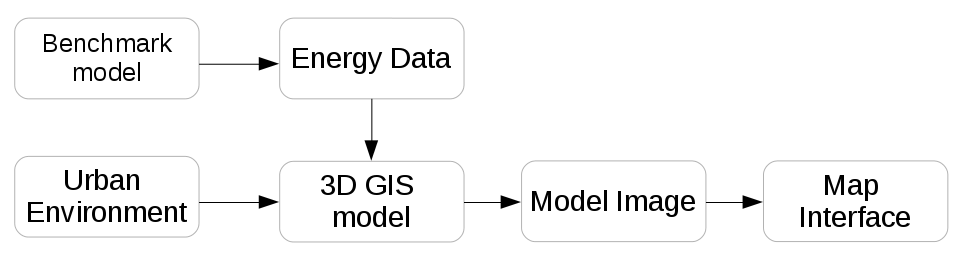
\includegraphics[width=0.7\linewidth]{flow.png}
  \caption{General Work Flow}
  \label{fig:flow}
\end{figure}

\subsection{Input}
\subsubsection{Energy Data}
The energy profile used in the study is retrieved from simulation
results of commercial building benchmark models developed by
U.S. Department of Energy (DOE)~\cite{DOE2015}. The building types
involved in the current project include: Large Office (LO), Medium
Office (MO), Small Office (SO), Stand-alone Retail (SR), Supermarket
(SU), Quick Service Restaurant (QR), Full Service Restaurant (FR),
Large Hotel (LH) and Midrise Apartment (MA). The two-letter shorthand
in the parenthesis after each building type is used in the building
label for the dynamic map and the box plot labels in
section~\ref{boxPlot}. The general information for the benchmark
buildings are shown in \tref{tab:doeModel}:

\begin{table}[h!]
  \centering
  \begin{tabular}{l|l|c|c}
    \hline
Building Type Name&Shorthand&  Floor Area (ft2)    & Number of Floors\\
    \hline
Large Office	         &LO&  498,588	      & 12\\
Medium Office	         &MO&  53,628	      & 3\\
Small Office	         &SO&  5,500	      & 1\\
Warehouse	         &WH&  52,045	      & 1\\
Stand-alone Retail       &SR&  24,962	      & 1\\
Strip Mall	         &SM&  22,500	      & 1\\
Primary School	         &PS&  73,960	      & 1\\
Secondary School         &SS&  210,887	      & 2\\
Supermarket	         &SU&  45,000	      & 1\\
Quick Service Restaurant &QR&  2,500          & 1\\
Full Service Restaurant  &FR&  5,500          & 1\\
Hospital	         &HO&  241,351	      & 5\\
Outpatient Health Care   &OP&  40,946	      & 3\\
Small Hotel	         &SH&  43,200	      & 4\\
Large Hotel	         &LH&  122,120	      & 6\\
Midrise Apartment        &MA&  33,740	      & 4\\
    \hline
\end{tabular}
\caption{DOE Benchmark Building General Information~\cite{DOE2015}}
\label{tab:doeModel}
\end{table}

The default setting of the benchmark models are stand-alone, but the
building in a community setting are imposed to influences from
surrounding buildings and the ``stand-alone'' assumption is not
realistic. To account for this issue, the model used in this study is
assumed to be within an urban context, thus the presence of
surrounding building should be reflected in the reference building
models. The general assumption used in this study is a 20ft exterior
shading on each side of each building.

\subsubsection{3D GIS Model}
The conceptual community model is constructed in
CityEngine~\cite{cityEngine2015}. CityEngine is a software developed
by Esri. It can aggregate geographic information into buildings and is
capable of smoothly transition models to ArcGIS\cite{ArcGIS2015}, one
of the widely applied tools for Geo-referenced data presentation and
analysis. Buildings in CityEngine is defined with ``rules'' using CGA
(Computer Generated Architecture) shape grammar that is unique to
CityEngine. The rule-based modeling of urban environment enables fast
construction and easy adjustability of urban density, skyline and
terrain control. It also enables easy aggregation of Energy profile
data into 3D urban environment models.

Although the urban environment in this study is a conceptual setting,
we still want it to reflect the topological and density pattern in a
real urban environment. To construct the model, we first extracted the
topological pattern from an existing urban design project, the Mellon
Arena Project~\cite{baird2014} (\fref{fig:mellonArena}.  There are
eight building types in the project: Residential (43\%), Town House
(2.9\%), Community Center (0.4\%), Commercial (3.8\%), Office (19\%),
Hotel (4.7\%), Cinema (1.4\%) and Garage (24.7\%).
\begin{figure}[h!]
  \centering
  \begin{subfigure}
  \centering
  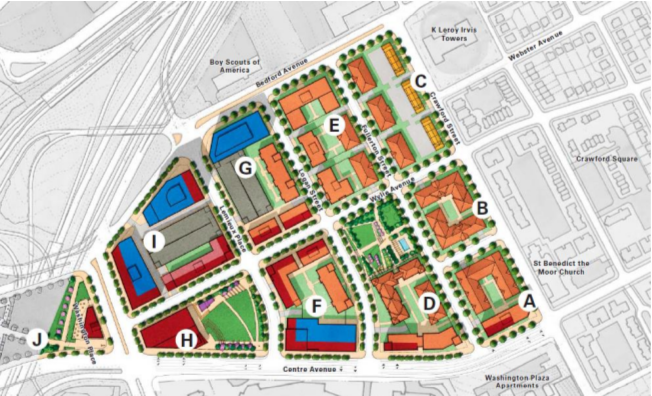
\includegraphics[width=0.5\linewidth]{mellonArena}
  \caption{Mellon Arena Project Site Plan View}
  \label{fig:mellonArena}
\end{subfigure}
~
\begin{subfigure}
  \centering
  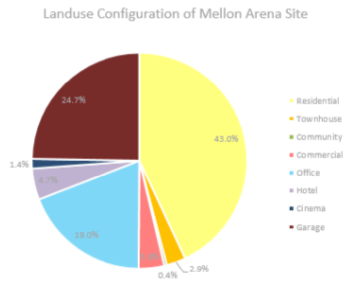
\includegraphics[width=0.3\linewidth]{mellonPie}
  \caption{Mellon Arena Site Land use Configuration}
  \label{fig:mellonPie}
\end{subfigure}
\end{figure}
The 16 building types in DOE commercial benchmark models do not
perfectly correspond to those in the Mellon Arena Site. In order to
adapt the topological pattern of the Mellon Arena Project, a mapping
(function) from building types of Mellon Arena Site to building types
of DOE models is created as is shown in \tref{tab:typeMap}.
\begin{table}[h!]
  \centering
  \begin{tabular}{c| c| c}
    \hline
    Mellon Arena Type &Probability &DOE Building Type\\
    \hline
    Hotel &50\%&Large Hotel\\
    \cline{2-3}
    &50\%&Small Hotel\\
    \hline
    Office &30\%&Large Office\\
    \cline{2-3}
    &30\%&Medium Office\\
    \cline{2-3}
    &30\%&Small Office\\
    \hline
    Residential &100\%&Midrise Appartment\\
    \cline{1-2}
    Townhouse &100\%&\\
    \hline
    Commercial &25\%&Full Service Restaurant\\
    \cline{2-3}
    $+$ Cinema $+$&25\%&Quick Service Restaurant\\
    \cline{2-3}
    Community &25\%&Super Market\\
    \cline{2-3}
    Center &25\%&Stand-alone Retail\\
    \hline
  \end{tabular}
  \caption{Mapping of Mellon Arena to Building Types of DOE benchmark model}
  \label{tab:typeMap}
\end{table}

The four major building sectors involved in the current project are
residential, commercial, office and hotel. Their topological pattern
is represented in Figure \ref{fig:mellonTop}. The conceptual model
construction follows the building type topological pattern and the
urban density as the Mellon Arena Project (\fref{fig:sitePlan})
\begin{figure}[h!]
  \centering
  \begin{subfigure}
  \centering
  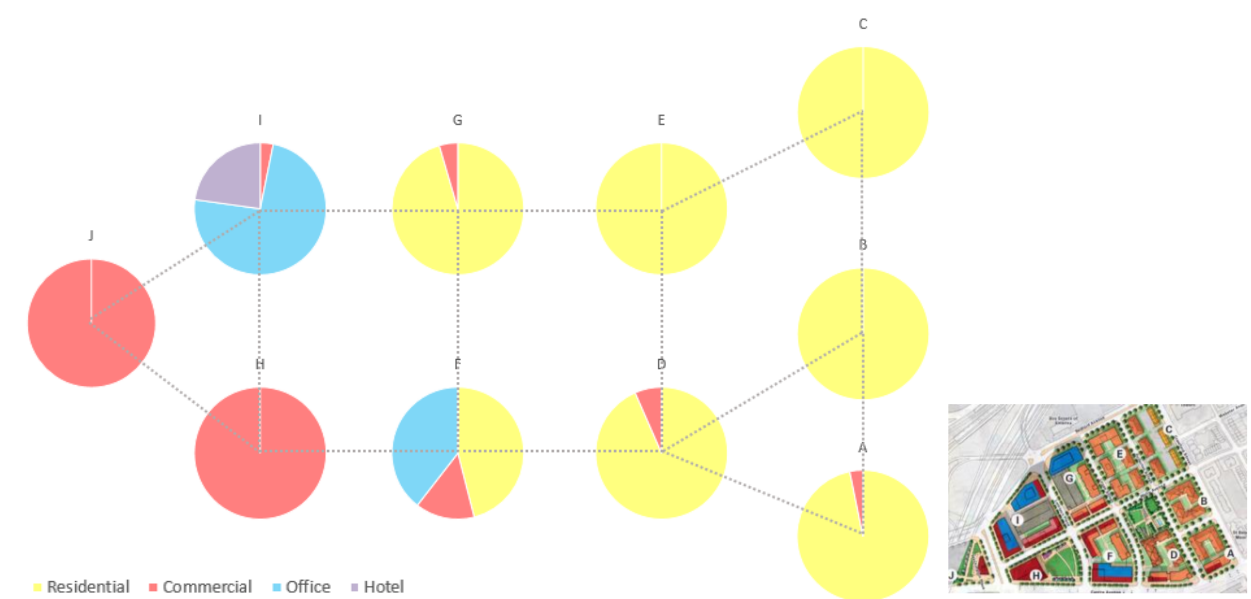
\includegraphics[width=0.7\linewidth]{mellonTop}
  \caption{Building Type Topological Pattern, Mellon Arena}
  \label{fig:mellonTop}
  \end{subfigure}
  ~
  \begin{subfigure}
  \centering
  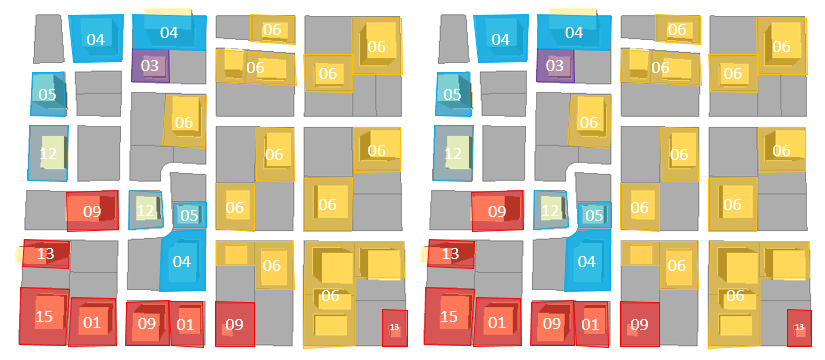
\includegraphics[width=0.7\linewidth]{sitePlan}
  \caption{Site Plan of Conceptual Model}~ (01: Full Service
  Restaurant, 03: Large Hotel, 04: Large Office, 05: Medium Office,
  \\06: Midrise Apartment, 09: Quick Service Restaurant, 12: Small
  Office, \\13: Stand-alone Retail, 15: Super Market)
  \label{fig:sitePlan}
  \end{subfigure}
\end{figure}   

\subsection{Data Collection and Analysis}
\subsubsection{Simulation Data Analysis of the benchmark
  models}\label{boxPlot}
The output of EnergyPlus simulation of 16 benchmark buildings are read
and processed with python script. This data loading and processing
module is used in both data analysis and the dynamic plot in the
interface design.

By analysing the simulation result of the Heating Energy (Gas) and the
Cooling Energy (electricity), we observed a large variation between
different building types.

Hourly heating demand of the benchmark building types involved in the
current model range from 0 to 12000 kBtu. The majority (75\%) of all
hourly consumption are below 2000 kBtu. All building types have a
large amount of outliers on the upper side. This indicates heating
demand of all building types are right skewed. The building type with
highest median heating demand are Large Hotel and Super Market. These
two building types could become the major ``heat sink'' or anchor load
building to be connected to a district system. In terms of peak
demand, Large Office has the highest peak heating demand
(\fref{fig:heatBox}).

Hourly cooling demand benchmark building types involved in the current
model range from 0 to 2500 kBtu, which is about 20\% of that of the
peak heating demand. Large Hotel has no outliers on the upper side,
meaning its hourly consumption are not as right skewed. Only Large
Hotel has non-zero median cooling demand (about 600 kBtu), meaning it
is the only building that has persistent cooling demand all year-round
. The design impact is: Large Hotel can act as an anchor building for
cooling if the central plant is a heating-cooling combined system that
can supply cooling energy as well. The consistent high cooling load of
Large Hotel also indicate a high portion of heat rejection. The reject
heat could be recovered and reused if building with moderate heating
demand are placed near the heavy cooling consumers
(\fref{fig:coolBox}).

The aggregated analysis above intends to provide a basic understanding
of the energy profile data distribution involved in the current
project. We anticipate to acquire more information than these
aggregated statistics with Dynamic Energy Map.

\begin{figure}[h!]
  \centering
  \begin{subfigure}
  \centering
  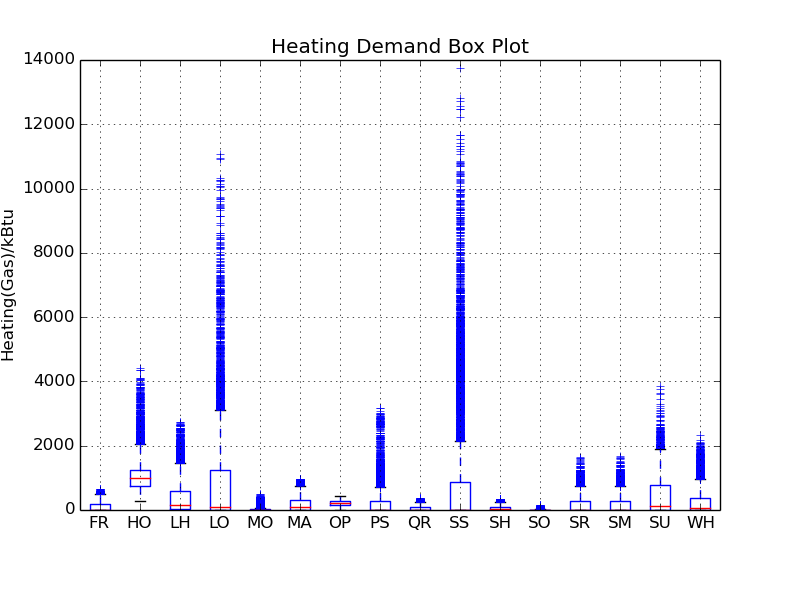
\includegraphics[width=0.7\linewidth]{heatBox}
  \caption{Heating Demand Box Plot}
  \label{fig:heatBox}
  \end{subfigure}%
  ~
  \begin{subfigure}
  \centering
  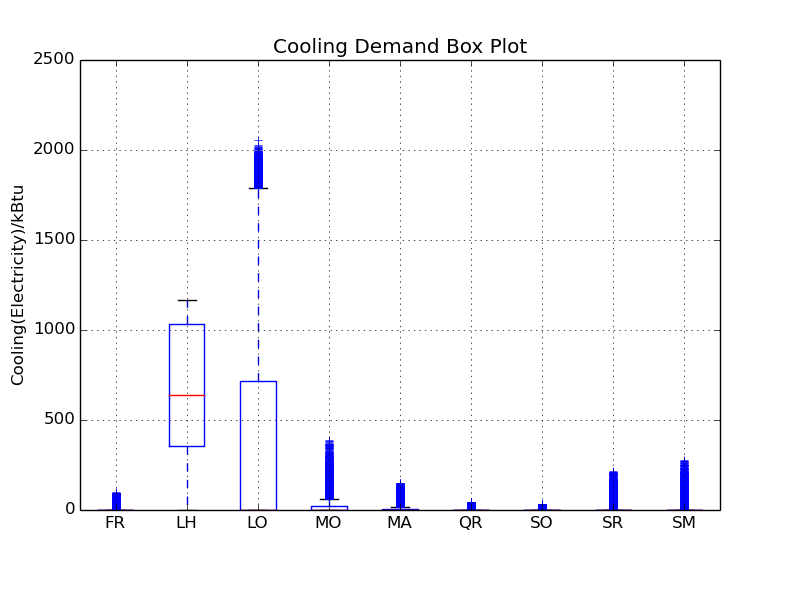
\includegraphics[width=0.7\linewidth]{coolBox}
  \caption{Cooling Demand Box Plot}
  \label{fig:coolBox}
  \end{subfigure}
\end{figure}   

\subsection{Temporal Data Aggregation}
The authors have experimented with two approaches to aggregate energy
profile data into the conceptual model constructed in CityEngine: 1)
write the energy profile data directly in the rule file for building
generation in CityEngine 2) importing 3D models from CityEngine to
ArcScene and aggregate the energy data into the 3D feature with
``one-to-many'' join.

The second approach has the advantage of 1) ready-to-use data
classification method and map symbol templates that facilitates
choropleth map design 2) the ``time-slider'' function for creating a
time-wise navigation and animated map. \fref{fig:arcgisTime} shows the
interface slider and the dynamic map of heating energy demand for the
conceptual model using ArcGIS. There are several problems of this
approach: 1) its high requirement of computational power makes it
infeasible to view on a normal PC. 2) The time dimension only exist
inside the map file. Although the animated map can be exported, the
output animation contains neither any form of temporal label nor the
control of playback. 3) For 3D GIS model, it does not contain a proper
function to extract single frames of map images, making it impossible
to implement exterior interface that deals with 3D maps.

The first approach, on the contrary, provides more flexibility but
also requires much user-end work including: pre-processing of energy
profile data, implementing data classification method and the
bivariate color ramp. An interface is also needed for visualising the
image sequence.

\begin{figure}[h!]
  \centering
  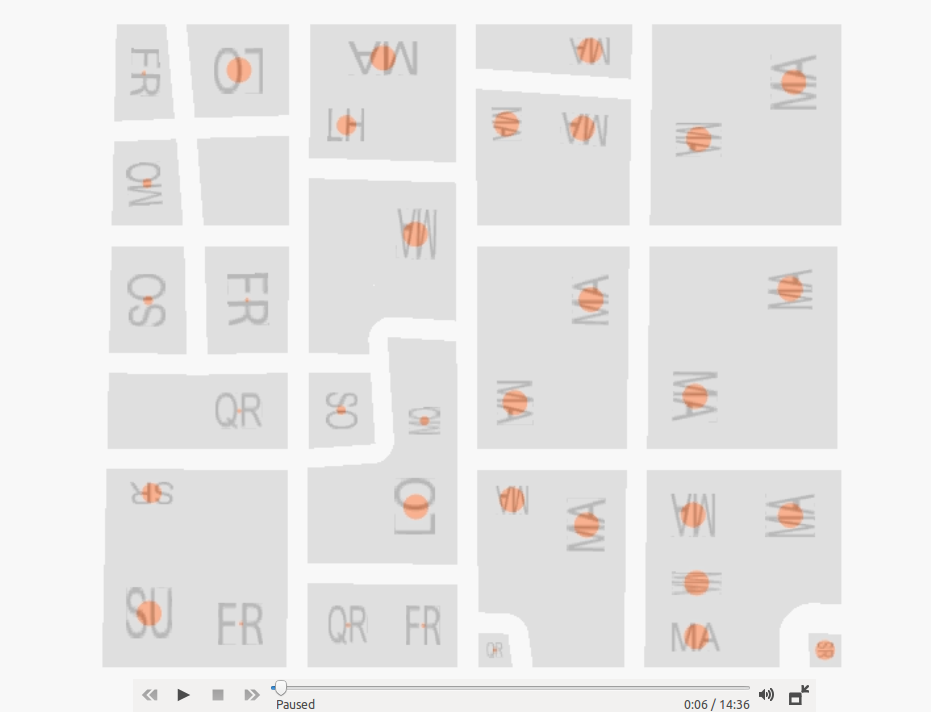
\includegraphics[width=0.5\linewidth]{arcgisTime}
  \caption{ArcGIS Time Slider for Temperal Data Display}
  \label{fig:arcgisTime}
\end{figure}

Due to limited time, the experimented GIS software are only restricted
to ArcGIS and CityEngine. There could be better alternatives to
achieve a dynamic map with more elegance. Find a better alternative
software to implement a dynamic map could be part of the work of the
next stage of the project.

\newpage
\subsection{Interface Specification}\label{interfaceSpec}
\subsubsection{User Definition}
We want to specify a user profile in order to best convey the
information with the Dynamic Energy Map.

The major category of user group for the Dynamic Map includes: 1)
policy makers, 2) urban planners with the interest in executing
community level energy strategys 3) researchers in energy related
fields 4) public groups or individuals that are involved or interested
in the decision making process of community energy planning.

The target user for the current interface design is restricted to
researchers in energy related fields. The assumption on this user
group about their skill level and background knowledge is that 1) they
have the basic ability to read and understand the layout of a map
environment and can associate it with the urban environment setting
they are associated with 2) they have the ability to correctly
understand moderately complicated map legend and data plot 3) they
have the basic understanding of related concept of building energy
performance attribute and the general implications of these
attributes. The assumptions about their intention is that they might
have different research interest and focus. These assumptions implies
the interface design should: 1) provide both qualitative and
quantitative information; 2) allow for some degree of user control
over data classification, legend selection and full control over time
navigation

\subsubsection{Goal Function}
The goal function of the interface is defined as: ``\textbf{Revealing
  the spatial-temporal heating and cooling demand variation of the
  conceptual model with Dynamic Energy Map}.''

As is mentioned in section \ref{districtDesign}, with the Dynamic
Energy Map that depict the spatial temporal load variation, one will
idealy be able to 1) idendify anchor load building, 2) conduct better
design of local load balancing, 3) identify energy recovery
opportunities of the following forms: an individual building with
mixed heating or adjacent buildings with opposite heating and cooling
demand.

\begin{enumerate}[1).]
\item Identify anchor load building
  
  To achieve this function, the map should be able to make the
  building with persistant high heating or cooling demand stand
  out. Thus the design of color scheme that assigns vibrant colors to
  high demand and white to low demand. The break points of ``high''
  demand remains to be decided in further project development. For the
  current implementation, the break point is acquired with quantile
  classification method with.

\item Local load balancing
  
  To achieve this, the first step would be to enable users to select a
  subset of the existing buildings and the program will calculate the
  aggregated maximum load and the load variation of the selected
  building group within the specified time period.

  The next step is to provide a utility that finds the optimal
  partition of the buildings in the urban environment that has the
  minimum load variance ratio within the group difference. A brute
  force approach would be:

  \begin{enumerate}[{Step }I.]
  \item Generate an adjacency table (dictionary) from the collection of
    building lot polygons with the key being building lot centroid labels.
  \item Create all legal partitions of the set of building centroids
    based on the adjacency table (i.e. a partition that includes a
    multi-part feature is not a legal partition)
  \item Calculate the sum of the load variation ratio for each of the
    legal partition. The load variation ratio for each subset of the
    element in a partition (a group of building) equals
    $${\text{max aggregated load} - \text{min aggregated load} \over \text{max aggregated
      load}}$$
  \item Find the partition with the minimum sum of load variation ratio
  \end{enumerate}
  
\item Identify energy recovery opportunities

  To achieve this, the heating and cooling demand should be
  represented on the same map that better depict the correlation.

\end{enumerate}

\subsubsection{Specification of the Major Operation}
The desired major operations for the target user include: 
\begin{itemize}
\item Map display and data plot
\item Navigation utilities that navigates through dynamic map and data
  plot
\item Provide default settings for choropleth map display
\end{itemize}

\paragraph{Map display and data plot}
For researchers or planners: The desired map display should be a 2D
and 3D map (providing easy toggle between 2D and 3D map or align the
two representations side by side) with graduated symbol or color
representing the heating or cooling demand. The map display should
also be coupled with corresponding data plot or data statistics that
providing the quantitative insight that supports design decisions.

For general public: The desired map display should be a 3D map
. Instead of using data plot, a more intuitive bar chart of the
aggregated demand could be more helpful in presenting a general
idea. The bivariate choropleth map legend should also be replaced with
two color ramps or even with only colors of extreme value. The data
classification method should also be chosen so that the peak
occurrence time is emphasized rather than the absolute energy
consumption value.

\paragraph{Navigation utilities that navigates through dynamic map
  and data plot}
The ability to navigate through a series of map images and present
dynamic data plot accordingly, is the basic function that differs
the current work from a static map. Some desired behavior of the
slider includes:
\begin{itemize}
\item Linear and cyclic time representation. According to section
  \ref{anime}, the time has both linear and cyclic aspect. The time
  navigation utility should provide both ``linear'' time navigation
  and ``cyclic'' time navigation. This requires a global time
  navigation that accounts for the linear aspect: it can go through
  the whole time period with the highest time resolution. It also
  requires a series of default time steps settings corresponding to
  the natural recurring pattern of the energy usage profile
\item Another desired feature is providing adjustable auto-play of the
  map animation. The reasoning behind this is the debatable level of
  user control in the study of Johnson and Nelson~\cite{Nelson1998},
  when they argue that allowing arbitrary time control might degrade
  the ability of animated map on conveying temporal pattern. This
  feature is to be implemented in future development of the project.
\end{itemize}

\subsubsection{Provide default settings for choropleth map display}
Creating several default settings for choropleth map display,
i.e. provide choices for data classification and color mapping. For
the current implementation, the variables in display is the heating
and cooling energy consumption profile. The customization choices only
restrict to the two classification method: even or quantile
method. The color ramp is predefined to be a bivariate color ramp from
white to red and blue. For later stages, a desired behavior would be
to provide the full control of color settings.

\subsubsection{Guidelines from Literature Study}
Here we summarizes some of the design choices made according to
related literature research on dynamic map design:
\begin{itemize}
\item Provide both 2D and 3D map display as a result of the debating
  situation mentioned in section \ref{2d3d}.
\item Choose bivariate choropleth map representation which has the
  highest accuracy rate in map reading experiments~\cite{Elmer2012}.
\item Providing the most commonly used data classification method:
  Equal Interval and Quantile Interval~\ref{dataClassification}
\item The number of classes for energy data classification is chosen
  to be 7, less than the suggested value of 10 as a result of smaller
  display size than 1024x768~\cite{doi:10.1559/1523040639298}
\item Provide both linear and periodical navigation based on section
  \ref{timeRepresent}
\item Using the principle of ``dual coding''~\cite{Resch2014} to
  assist legend reading by section \ref{anime}.
\item Noise removal in map display of energy profile
  data~\cite{Dorling1992}. This is done through the discrete color
  scheme design.
\end{itemize}

\subsection{Interface Design}\label{interfaceDesign}
\subsubsection {General Layout}
The interface for dynamic map display includes three major sections: a
series of sliders for controling images are on the left and the data
plot of energy profile of building sectors and aggregated demand are
on the right.

The main window on the top left is used for displaying the 2D dynamic
map of the conceptual model. The lower left of the window displays the
current time for the image and dynamic plot in display. The lower left
section contains a series of sliders for controling interactive
navigation of image and plot sequences. The right hand side of the
interface contains the dynamic data plot of the four major building
sectors: Hotel, Office, Residencial and Commercial buildings. The
lower right are the aggregated heating / cooling demand profile for
the whole site. The left column are the heating energy consumption in
natural gas and the right column are the cooling energy consumption in
electricity. On the lower right there are four buttons providing two
default forward and backward navigation, 1h and
24h. (\fref{fig:interfaceLayout}).
\begin{figure}[h!]
  \centering
  \begin{subfigure}
  \centering
  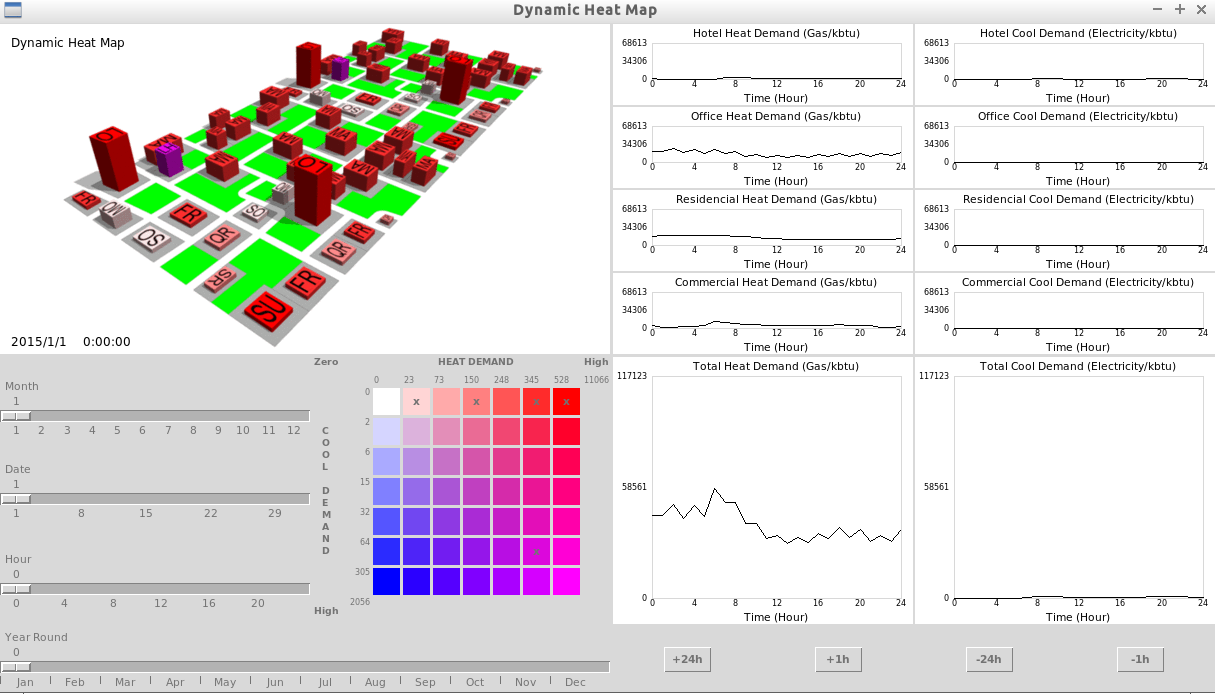
\includegraphics[width=0.7\linewidth]{interface0720}
  \caption{Dynamic Map Interface Layout (3D map)}
  \label{fig:interface0720}
\end{subfigure}
~
\begin{subfigure}
  \centering
  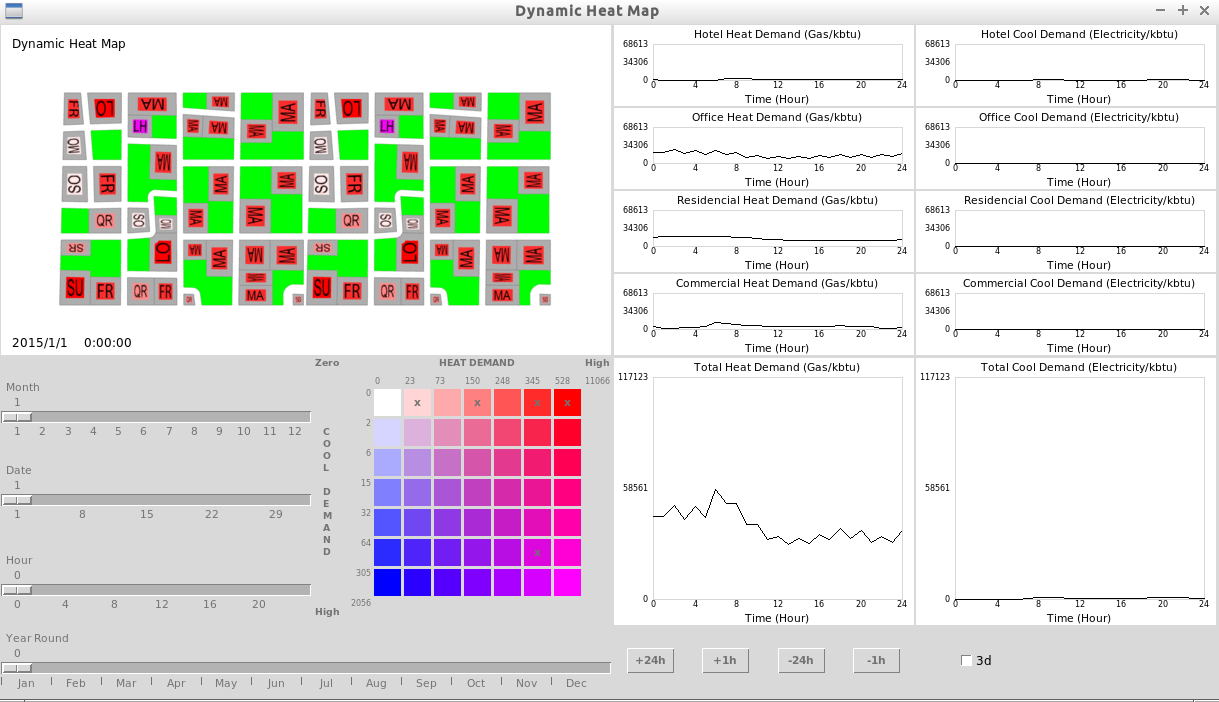
\includegraphics[width=0.7\linewidth]{interface2d}
  \caption{Dynamic Map Interface Layout (2D map)}
  \label{fig:interface2d}
\end{subfigure}
\caption{Dynamic Map Interface Layout}
\label{fig:interfaceLayout}
\end{figure}
Between the aggregated heat demand and the sliders, there is a
choropleth legend. According to section \ref{anime}, the comparison of
the map and the legend becomes tricky for dynamic maps. In order to
assist this task, tick marks of ``x'' are added to the legend to
indicate the color appeared in the map \fref{fig:legend}.
\begin{figure}[h!]
  \centering
  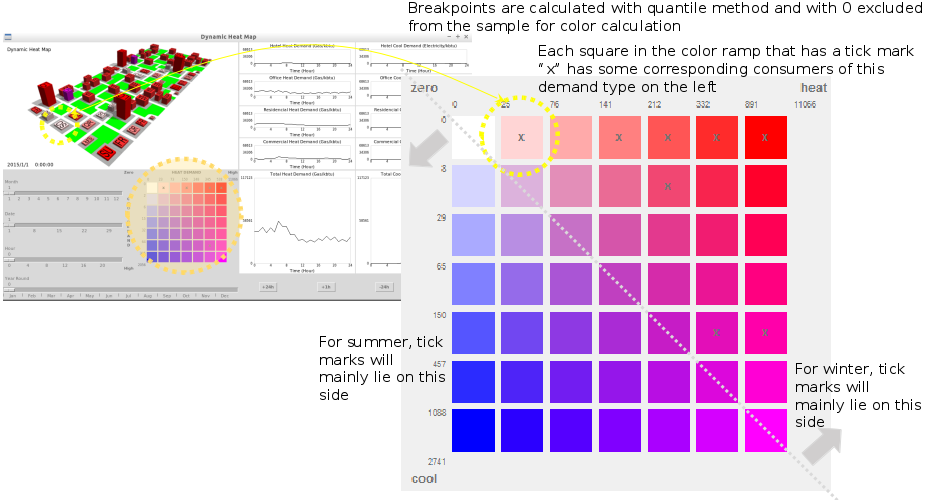
\includegraphics[width=0.7\linewidth]{legend}
  \caption{Bivariate Color Legend with Tick Mark Indicators}
  \label{fig:legend}
\end{figure}
\subsubsection {Navigation Function}
The navigation function is achieved with the four slider and the four
buttons above the sliders on the lower left of the window. The top
slider labeled with ``Year round'' has a range of 0 to 8760 (not
inclusive). the change of 1 in the slider position corresponds to the
change of 1 hour in time, which results in the display of the image of
the next or previous hour in time. The slider labeled with ``month''
has a range of 1 to 12, which corresponds to the 12 months in year,
the change of the month slider results the jump of 1 month forward or
backward in time. This function is intended to provide easy comparison
of montyly variation of the energy consumption behavior. Similarly,
the change of the ``date'' and ``hour'' slider corresponds to the time
change of one day or one hour respectively. The four buttons provides
a separate control intended to provide micro level adjustment of time.

\subsubsection {Dynamic Plot}
The input images to the main window is generated from the CityEngine
model. The graph is ploted by reading in simulation data from
EnergyPlus. The starting point (left end) of the plot corresponds to
the position indicated by the slider. 

\subsubsection {Implementation tools and strategy}
The softwares or platform involved in the project include EnergyPlus
for building simulation, CityEngine for 3D modeling and image
generation, Python 2.7 for interface design. The interface is written
in Python2.7 with standard Tkinter graphic package including the data
plot section.

\section{Case Analysis: Using the Current Dynamic Map to Design a District Energy System}
This section uses the tool assist the design of a district energy
network. The common steps in conducting such a design follows the
guidance of ~\cite{IDEA2012}. The goal of the case study is to
demonstrate how dynamic energy map can do better than static map in
assist the design of a district system and in demonstrating the
advantage of a district system. The major performance metric comparing
the static and dynamic map is the energy throughput.

As is suggested in the document~\cite{IDEA2012}, the data needed for
designing a district system include: 1) existing and emerging thermal
energy consumption, 2) fuel source availability and 3) land use
constraint. For the current case analysis on the conceptual setting,
the energy consumption is restricted to the heating gas energy
consumption and cooling electricity energy for the existing buildings.
The assumption about the central plant is it uses natural gas to
produce electricity, as is the most common case. It can also produce
chilled water with absorption chiller in summer. For land use
constraint, we assume the pipeline can be put only under the road
network.
 
\section{Findings and Discussion}
\subsection{Landuse Design on Load Balancing}

One of the point of having a visualization of dynamic map is, as
Dorling and Openshaw suggested, to detect mistakes that could
otherwise be neglected under a black box calculation routine or some
false application of rule of thumbs~\cite{Dorling1992}.

\grey{not finished}
\section{Conclusion}
  \begin{enumerate}[label*=\arabic*.]
  \item Summary of the current approach in implementing the dynamic
    Energy Map
  \item Limitations of the current implementation
    \begin{enumerate}[label*=\arabic*.]
    \item Simplified building simulation assumption about urban
      environment
    \item Lack of user choices for the stand-alone user interface as a
      result of its dependence on existing modeling softwares
    \end{enumerate}
  \item Future Expansion of the project
    \begin{enumerate}[label*=\arabic*.]
    \item Adding information of the supply side: residual energy,
      sustainable energy
    \item Providing different interfaces for different user population
    \item 2D and 3D compatible \\The reason for providing 2D map
      together with 3D map is that 2D maps have the following good
      properties:
      \begin{enumerate}[label*=\arabic*.]
      \item Better for region selection and spatial navigation than 3D
        map
      \item Better for conveying spatial relationship that does not
        involve height induced variation
      \item For larger scale display of city, state or nationwide, 3D
        building geometries becomes less significant in providing the
        urban environment context
      \end{enumerate}
    \item Creating an on-line tool for better information share
      \begin{enumerate}[label*=\arabic*.]
      \item Potential techniques: see 2.4
      \end{enumerate}
    \end{enumerate}
  \end{enumerate}
\item Acknowledgments
\end{enumerate}
\newpage

\begin{figure}[h]
  \centering
  \begin{subfigure}
  \centering
  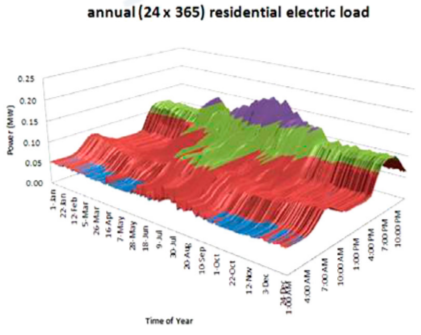
\includegraphics[width=0.4\linewidth]{resi}
  \caption{Residential Building Electricity Demand~\cite{baird2014}}
  \label{fig:resi}
\end{subfigure}
~
\begin{subfigure}
  \centering
  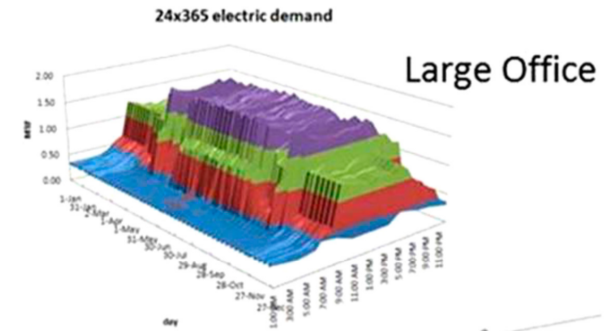
\includegraphics[width=0.4\linewidth]{office}
  \caption{Office Building Electricity Demand~\cite{baird2014}}
  \label{fig:office}
\end{subfigure}
\end{figure}

\begin{abstract}
  This document provides an approach of creating a space-time Energy
  Map, or a Dynamic Energy Map. The approach is demonstrated with a
  conceptual urban environment setting created in CityEngine based on
  the extracted topological and density pattern from an existing urban
  design project. The buildings in the conceptual model is then
  assigned an energy profile of certain DOE Commercial Benchmark
  Building Reference model based on its building type. Hourly energy
  heating and cooling demand profile are then obtained from the
  EnergyPlus simulation of DOE Commercial Benchmark models. The energy
  consumption data is classified into groups with consideration of
  \red{building energy design context} and the data distribution
  properties. A corresponding color coded energy profile is then
  generated and imported to CityEngine. 8760 color coded 2D and 3D map
  images was then extracted from CityEngine with Python script. A
  series of data reading, plotting, data classification and
  color-coding calculation utilities were implemented. An interactive
  interface for visualizing the images and dynamic data plot with
  sliders is implemented using Python. The tool is anticipated to
  provide decision insight for community energy management and
  planning, demand-side strategy design and district system sizing.
  
  The document will also briefly discuss one of the test-bed for data
  classification and visualization.

\end{abstract}
\end{comment}

\newpage
\bibliographystyle{plain}
\bibliography{myCitation}
\end{document}